\section{Diseño y funcionamiento final}
Luego de todo el desarrollo de la aplicación mostraré el diseño y funcionamiento final que tiene.

\subsection{Inicio de sesión y registro de usuario}
\begin{figure}[h]
    \centering
    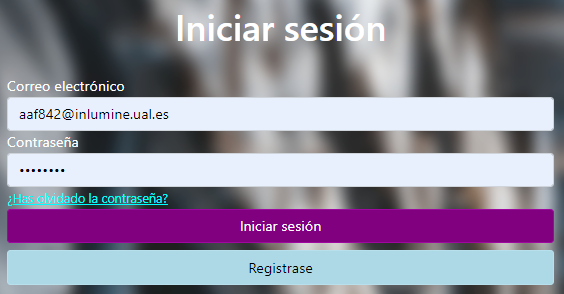
\includegraphics[scale=0.5,keepaspectratio]{../contruccion_aplicacion/design/login.png}
    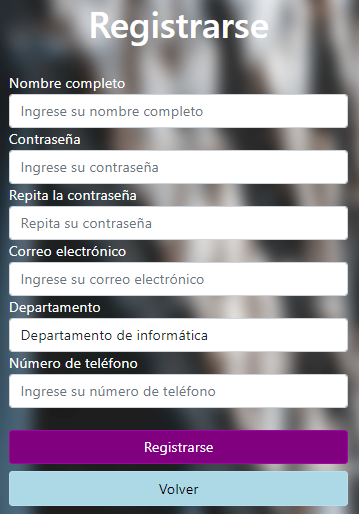
\includegraphics[scale=0.5,keepaspectratio]{../contruccion_aplicacion/design/register.png}
    \caption{A la izquierda el inicio de sesión y a la derecha el formulario de registro de usuario}\label{fig:register-and-login}
\end{figure}
En la figura \ref{fig:register-and-login} podemos ver cómo ha quedado el resultado final de nuestro registro e inicio de sesión de Inventarium. Dentro del cuadro de inicio de sesión se añade un enlace posibilitando una recuperación de la contraseña. Dicha recuperación tendría que ser facilitada por un técnico. En el complemento del trabajo de fin de grado junto a la implementación del gestor de correos completaremos la funcionalidad para que un usuario pueda recuperar sus credenciales.
\\Dentro del formulario de registro todos los campos deben ser rellenados de forma obligatoria. Además se han implementado comprobaciones para que estas variables cumplan con unas determinadas propiedades:
\begin{itemize}
    \item El campo del nombre completo debe contener más de ocho caracteres
    \item La contraseña debe tener más de ocho caracteres
    \item La entrada de ``Contraseña'' y la de ``Repita contraseña'' deben ser iguales
    \item El correo electrónico tiene que tener la extensión \textbf{@ual.es} o \textbf{@inlumine.ual.es}
    \item El apartado para ingresar el número de teléfono debe contener 9 dígitos exactos.
\end{itemize}
\section{Distribución de componentes y diseño}
El desarrollo de los componentes se ha hecho pensando fírmemente en la modularización de los mismos.

\subsection{Componentes principales}
Estos componentes reciben su nombre debido a que son la estructura principal de la aplicación. Son los átomos que conforman los distintos componentes.
\\Un ejemplo sería la figura \ref{fig:user-view}. En ella podemos ver cómo se muestran los campos que puede contener un usuario, el correo electrónico, el departamento al que pertenece, su número de teléfono y qué tipo de usuario es.
\begin{figure}[h]
    \centering
    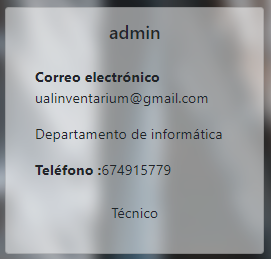
\includegraphics[scale=0.5,keepaspectratio]{../contruccion_aplicacion/design/user.png}
    \caption{Representación de un usuario en la aplicación}\label{fig:user-view}
\end{figure}
Este componente ha sido creado en base a uno principal con el cual también podríamos crear el de la figura \ref{fig:user-unit}.
\begin{figure}[h]
    \centering
    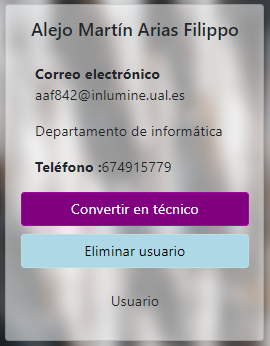
\includegraphics[scale=0.5,keepaspectratio]{../contruccion_aplicacion/design/user_unit.png}
    \caption{Representación de un usuario y posibles acciones sobre él en la aplicación}\label{fig:user-unit}
\end{figure}
¿Qué objetivo pretendo conseguir con esta diferenciación? En la modularización del código, es decir, en una separación entre visualización y acciones posibles sobre el objeto.
\\Es decir, esta vista donde se proyecta la visualización del usuario podemos ponerla en varias secciones del código pero, dónde podemos modificar su campos. No se pretende posibilitar la modificación de los campos en todos los sitios donde se llame al componente. Por ello creo el concepto de vistas unitarias.
\\En una vista unitaria se van a poder realizar todas las acciones posibles sobre un objeto. Esto nos ayudará a poder hacer una separación de permisos, dependiendo de si es un usuario o un técnico y a implementar modificaciones únicamente en un sitio en caso de realizar algún cambio. Por ejemplo el usuario de la figura \ref{fig:user-unit} es de la vista unitaria del usuario. Dentro de ella podemos realizar diferentes acciones como convertirlo en técnico o eliminarlo.
\\Esta diferencia de vistas nos permite crear relaciones que nos ayudarán en la gestión de la herramienta. Las vistas unitarias junto a sus respectivas relaciones son las siguientes:

\subsubsection{Usuario}
Dentro de un usuario dispondremos de un campo donde podremos acceder para visualizar sus préstamos. También podremos realizar diferentes acciones sobre él en caso de que seamos un usuario \textit{técnico}:
\begin{itemize}
    \item Dar de alta
    \item Eliminar
    \item Convertir en técnico
\end{itemize}

\subsubsection{Objeto}
En el objeto podremos acceder a un apartado donde veremos sus préstamos. También veremos al grupo de objetos al que pertenece y por último tendremos un campo donde podremos añadirle una configuración.

\subsubsection{Grupo de objeto}
Dentro de los grupos de objeto

\subsubsection{Préstamos}